
\documentclass[12pt]{article}%
\usepackage{amsmath}%
\usepackage{amsfonts}%
\usepackage{amssymb}%
\usepackage{graphicx}
\usepackage{booktabs}
\usepackage[utf8]{inputenc}
\usepackage{anysize}

\marginsize{2cm}{2cm}{2cm}{2cm} 
\begin{document}

\thispagestyle{empty}

\begin{center}
PONTIFICIA UNIVERSIDAD CATÓLICA DE VALPARAÍSO\\
FACULTAD DE INGENIERÍA\\
ESCUELA DE INGENIERÍA INFORMÁTICA\\

\vspace{4cm}

\Large{\textbf{Diagnosticador de severidad de fallos de rodamientos bajo velocidades variables utilizando la transformada de Fourier y Deep learning}}

\vspace{3cm}

\normalsize{\textbf{Sebastián Ignacio López Norambuena}}\\
\end{center}

\vspace{3cm}
\begin{center} 
Profesor guía: \textbf{Nibaldo Rodríguez Agurto}
\end{center}
\begin{center} 
Profesor co-referente: \textbf{Guillermo Cabrera Guerrero}
\end{center}
\vspace{1cm}
\begin{center} 
Noviembre, 2017
\end{center}
\newpage
\pagenumbering{roman}

\noindent
\Large{\textbf{Resumen}}\\

\normalsize
\noindent El rodamiento es uno de los componentes más utilizados en la maquinaria rotativa. Las fallas en estos elementos son muy comunes y tienen un gran impacto en la cadena de producción de una planta. Por lo tanto, es importante estudiar la tecnología de diagnóstico de fallas en rodamientos e incluirla en los planes de mantenimiento. Una señal de vibración perteneciente a un rodamiento, transporta información dinámica sobre el estado estado de salud de este; así que puede ser utilizada para identificar y clasificar fallas en la estructura de los rodamientos. Para automatizar este proceso, la ingeniería ha propuesto algoritmos de \textit{machine learning} que combinados con técnicas de extracción de características; entregan un diagnóstico óptimo sobre el estado de los rodamientos. Para mejorar el rendimiento de estos modelos cuando la dimensión de los datos de entrada es muy alta, se incluyen técnicas de reducción de dimensionalidad o selección de características. En este documento se propone utilizar esta combinación de técnicas de extracción de características y algoritmos de \textit{deep learning} que reducen la dimensionalidad y realizan un diagnostico de la salud del rodamiento. En la etapa de extracción, se aplicará la transformada rápida de Fourier a una señal de vibración; para obtener la magnitud de los coeficientes y emplearlos como características. Posteriormente una red neuronal profunda compuesta por dos sparse autoencoders y una capa de neuronas con la función de activación softmax, se encargarán diagnosticar la salud del rodamiento.
\newline

\noindent
\textbf{Palabras Clave:} rodamientos, diagnóstico, mantenimiento, señal de vibración, deep learning.

%----------------------Tabla de contenidos-----------------------------%

\newpage
\renewcommand{\contentsname}{Índice}
\renewcommand{\tablename}{Tabla} 
\tableofcontents
\renewcommand{\figurename}{Figura}
\renewcommand{\refname}{Referencias}
\renewcommand{\listtablename}{Lista de Tablas}
\newpage

%----------------------Tabla de contenidos-----------------------------%

%-------------------------Tabla de imagenes--------------------------%

\renewcommand{\listfigurename}{Lista de Figuras}
\listoffigures
\listoftables
\newpage

%-------------------------Tabla de imagenes--------------------------%

\pagenumbering{arabic}
\section{Introducción}

\paragraph{}
La maquinaria rotativa es ampliamente utilizada en muchos campos industriales y en los últimos años, el monitoreo de condiciones de estas máquinas ha cobrado especial importancia en el mantenimiento moderno. Lo anterior se ha debido, principalmente a la necesidad de reducir los tiempos de inactividad no programados y los costos asociados al mantenimiento, de manera que se pueda mantener la competitividad corporativa \cite{seeraa}. Así, con el monitoreo de condiciones se pueden detectar tempranamente fallas potencialmente desastrosas, reduciendo el tiempo de inactividad total de la máquina y de operaciones enteras.

\paragraph{}
Las técnicas de mantenimiento predictivo han demostrado ser estrategias eficaces para reducir fallas inesperadas en la maquinaria. El monitoreo de vibraciones es la tecnología de mantenimiento predictivo más utilizada \cite{zhan}, debido a la cantidad significativa de información que porta la señal sobre el estado salud de la maquinaria. Considerando que los rodamientos son un componente encontrado frecuentemente en la maquinaria rotativa y que pueden causar alrededor del 40-50\% \cite{issam} de todos los desperfectos, muchas investigaciones se centran en el monitoreo de vibraciones para estos componentes.

\paragraph{}
Los rodamientos giran constantemente en condiciones ambientales severas tales como alta temperatura, velocidad de rotación variable y grandes cargas, por lo que presentan una alta frecuencia de rotura \cite{fu}. Realizar un diagnóstico efectivo para los rodamientos es complejo, porque usualmente la señal de vibración tiene un comportamiento no lineal y no estacionario \cite{li}. Este comportamiento de la señal es consecuencia de la compleja estructura mecánica del rodamiento y sus duras condiciones de trabajo.

\paragraph{}
Los sistemas de monitoreo de condiciones son usados para obtener datos en tiempo real de las máquinas. Por lo tanto, enormes colecciones de datos son adquiridas después de un prolongado funcionamiento de estas máquinas. Como los datos generalmente se recopilan más rápido de lo que se tarda en analizarlos, existe la necesidad de un método de diagnóstico que sea capaz de analizar grandes volúmenes de datos y de realizar automáticamente un diagnóstico preciso.

\paragraph{}
Este tipo de métodos se denominan \textit{métodos inteligentes de diagnóstico de fallas} y en general, están compuestos por dos etapas. La primera consiste en extraer características útiles desde los datos recolectados con alguna herramienta de procesamiento de señales. La segunda utiliza técnicas de inteligencia artificial para distinguir el estado de salud de la maquinaria en base a las características obtenidas en el paso anterior.

\paragraph{}
La primera de estas etapas resulta clave en el diagnóstico de fallas para maquinaria rotativa \cite{guo}, porque reduce la dimensión de los datos, afecta directamente el reconocimiento de patrones y, por lo tanto, la calidad del diagnóstico. Los métodos convencionales de extracción de características incluyen técnicas en el dominio del tiempo, dominio de la frecuencia y tiempo frecuencia. Diversos autores utilizan estadísticos basados en la forma de la onda en el dominio del tiempo, tales como el valor pico, la media cuadrática, el factor de cresta, el índice de curtosis y la asimetría \cite{zhu}.
 
\paragraph{}
Los principales métodos en el dominio de la frecuencia corresponden a: el cálculo del espectro energético de Fourier \cite{jia}, el espectro de potencia \cite{li} y el análisis cepstral. Respecto a las  técnicas de tiempo frecuencia, suelen ser utilizadas la transformada de Fourier de tiempo corto (STFT), la distribución Wigner-Ville (WVD) y la transformada de paquetes wavelet (WPT). También es posible encontrar otros métodos basados en procesamiento de señales como la descomposición modal empírica (EMD) \cite{yu}, funciones modales intrínsecas (IMF), la transformada wavelet discreta (DWT), la transformada wavelet (WT) \cite{chang} y la transformada Hilbert-Huang (HHT) \cite{rai}.

\paragraph{}
Respecto a las técnicas de inteligencia artificial, aplicadas como clasificador en este contexto, podemos encontrar redes neuronales artificiales (ANN) \cite{ali}, máquinas de vectores de soporte (SVM) \cite{konar}, sistemas Adaptativos de inferencia neuro difusa (ANFIS) \cite{issam}, redes neuronales wavelet (WNN) \cite{wu} y otros. En la actualidad existe una tendencia en el uso de técnicas de \textit{deep learning}.

\paragraph{}
De acuerdo a Jia et al. (2016) \cite{jia}, los métodos inteligentes de diagnóstico de fallas más comunes emplean ANN's en el segundo paso, dando lugar a dos grandes desventajas. La primera es que la extracción de características depende de la experiencia en procesamiento de señales de los investigadores y se seleccionan según un problema de diagnóstico específico, por lo que probablemente no sean aptas para otros problemas. Y la segunda es que las ANN's utilizadas en estos métodos carecen de arquitecturas profundas, limitando la capacidad de estas para aprender las complejas relaciones no lineales en los problemas de diagnóstico de fallas.

\paragraph{}
Por lo tanto, es necesario extraer de forma adaptativa características ocultas en las señales de vibración que reflejen las diferentes condiciones de salud de la maquinaria, en lugar de extraer y seleccionar las características de forma manual. Las técnicas de \textit{deep learning} tienen el potencial de superar las deficiencias previamente mencionadas que poseen los métodos inteligentes de diagnóstico de fallas. Gracias a las arquitecturas profundas, las redes neuronales profundas (DNN) pueden capturar de forma adaptativa la información representativa de datos brutos a través de múltiples transformaciones no lineales y aproximar complejas funciones no lineales con un pequeño error.

\paragraph{}
En función de lo anterior, en el presente trabajo se propone un método inteligente de diagnóstico de fallas para rodamientos con la transformada de Fourier como técnica de extracción de características, y una DNN como clasificador. La red neuronal profunda utilizará \textit{sparse} autoencoders apilados para reducir la dimensión de las características a la vez que realizan un pre entrenamiento de las capas ocultas de la red. Además, se propone construir conjuntos de datos separados por velocidad, su respectiva carga, 3 severidades de falla para cada componente y un conjunto con todas las velocidades y cargas juntas.

\newpage
\section{Definición de objetivos}
\paragraph{}
En esta sección se definen los objetivos general y específicos que persigue la ejecución de este proyecto.
\subsection{Objetivo general}
\paragraph{}
Desarrollar un diagnosticador de severidad de fallos de rodamientos, bajo velocidades variables utilizando la transformada de Fourier discreta.

\subsection{Objetivos específicos}
\paragraph{}
Los objetivos específicos de este proyecto son los siguientes:
\begin{enumerate}
\item{Descomponer señales de vibración con la transformada de Fourier discreta.}
\item{Diseñar e implementar un algoritmo de \textit{deep learning} con sparse autoencoders.}
\item{Evaluar la exactitud del diagnosticador con 4 estados de salud del rodamiento.}
\item{Evaluar la exactitud del diagnosticador con 10 estados de salud del rodamiento.}
\end{enumerate}

\section{Plan de trabajo}
\paragraph{}
Este plan de trabajo utiliza los objetivos específicos como una base, debido a que estos explican las tareas que se deben llevar a cabo para cumplir el objetivo general. Esta segunda entrega, contempla la implementación del modelo propuesto y la evaluación del rendimiento de este. Para la próxima entrega se habrá pulido el marco teórico y la redacción de la investigación en general, sobre todo la discusión de resultados y el estado del arte.

\section{Marco Teórico}
\paragraph{}
Esta sección tiene como objetivo presentar antecedentes, conceptos, definiciones y la importancia de las técnicas y herramientas que se utilizarán en el desarrollo de esta investigación. Así, comenzaremos con el empleo de enfoques en el dominio de la frecuencia, seguido del aprendizaje profundo y luego el sustento matemático de ambos. Finalmente se dará a conocer la descripción del método inteligente de diagnóstico propuesto en esta investigación y todo lo relacionado con funcionamiento de la DNN como clasificador.

\paragraph{}
En la literatura especializada, existen antecedentes que sirven como base para esta investigación, un ejemplo de estos es Mao et al. (2017) \cite{mao}, quien utiliza la transformada de Fourier para extraer características de una señal y usar la energía contenida en el espectro de frecuencias como entrada de 3 clasificadores: una ANN,  una DNN con autoencoders apilados y una máquina de aprendizaje extremo (ELM). Este ejemplo corresponde a un  antecedente idóneo para esta investigación, debido a que implementa la misma técnica de extracción de características y clasificador que este trabajo, con la salvedad que sus autoencoders no incluyen la dispersión de los nodos en la capa oculta, variación denominada \textit{sparse} autoencoder y que sí es utilizada en esta investigación.

\paragraph{}
Otro ejemplo de un antecedente es Gupta et al. (2017) \cite{kanpaj}, quien postula que el análisis espectral es el enfoque más utilizado para detectar fallas en los rodamientos. El principal motivo de lo anterior es que los enfoques en el dominio del tiempo solo pueden detectar cuándo ocurre una falla en el rodamiento, mientras que el análisis espectral, además puede determinar en qué componente del rodamiento se encuentra el desperfecto. El autor también aclara que la transformada rápida de Fourier (FFT) es el algoritmo computacional más eficiente para convertir una señal en el dominio del tiempo a componentes de frecuencia discretos.

\paragraph{}
En cuanto a las redes neuronales profundas, podemos encontrar a Zhang et al. (2017) \cite{ran}, este autor  propone el uso de una DNN cuya función de costos es la entropía cruzada de los valores de salida y el \textit{target}. Los autores no utilizan métodos de extracción de características y solo dividen en segmentos la señal original para entrenar a la red neuronal profunda. Su principal argumento es que se debe mantener la coherencia temporal de la señal, pero la cantidad de datos que recibe la red es enorme, resultando en grandes tiempos de entrenamiento y una gran capacidad de cómputo.

\paragraph{}
A continuación se encuentran los conceptos y definiciones matemáticas de las herramientas que se utilizarán en esta investigación, comenzando por la transformada de Fourier y sus variantes, seguido del \textit{deep learning} (o aprendizaje profundo), los autoencoders y su variante \textit{sparse} autoencoder.

\subsection{Transformada de Fourier}
\paragraph{}
La transformada de Fourier es una herramienta matemática poderosa, por lo que es utilizada en diversos campos de la ciencia y la ingeniería. Puede ser vista como la transformación de una señal en un dominio (típicamente tiempo o espacio) a otro dominio, el dominio de la frecuencia. Al aplicar la transformada de Fourier a una señal, se obtienen sus componentes fundamentales en frecuencia que a menudo revelan estructuras ocultas, que en el dominio del tiempo, no son posibles de observar.

\paragraph{}
Como consecuencia de lo anterior, el análisis de Fourier está en la base de muchas teorías de la ciencia y juega un papel fundamental en el diseño práctico de la ingeniería. El alcance actual de la influencia del análisis de Fourier está indicado por una lista parcial de científicos e ingenieros que la utilizan \cite{robert}:

\begin{itemize}
\item{Los ingenieros de audio utilizan técnicas de Fourier, en parte porque el oído parece ser sensible al comportamiento del dominio de frecuencia.}
\item{Los estadísticos y probabilistas caracterizan y calculan las distribuciones de probabilidad usando transformadas de Fourier. Las transformadas de Fourier de las funciones de covarianza se utilizan para caracterizar y estimar las propiedades de los procesos aleatorios.}
\item{Los radioastrónomos utilizan la transformada de Fourier para formar imágenes a partir de datos interferométricos recogidos por arreglos de antenas.}
\item{Los cristalógrafos encuentran las estructuras cristalinas usando transformadas de Fourier de los patrones de difracción de rayos X.}
\item{Los ingenieros biomédicos recogen datos en el dominio de la frecuencia y luego los transforman
inversamente con Fourier para obtener imágenes de resonancia magnética.}
\end{itemize}

\subsubsection{Transformada de Fourier continua}
\paragraph{}
La transformada de Fourier continua es resultado de la generalización de las series de Fourier. Puede aplicarse prácticamente a cualquier función, no requiere que la función sea periódica, y para datos discretos, puede ser evaluada rápidamente usando una técnica moderna llamada transformada de Fourier Rápida (FFT). La transformada de Fourier de una función $f(t)$ se define \cite{anthony} como:

\begin{equation}
F(\omega)=\int_{-\infty}^{\infty}f(t)e^{-i{\omega}t}dt
\end{equation}

\paragraph{}
Donde $\omega$ es igual a la frecuencia angular $2{\pi}f$, y $F(\omega)$ es una función continua de valores complejos. Una vez que se ha determinado una transformada de Fourier, la función original $f(t)$ puede ser recuperada a partir de la transformada de Fourier inversa:

\begin{equation}
f(t)=\frac{1}{2\pi}\int_{-\infty}^{\infty}F(\omega)e^{i{\omega}t}d\omega
\end{equation}

\subsubsection{Transformada de Fourier discreta}

\paragraph{}
La transformada discreta de Fourier (DFT) (Ecc. \ref{dft}), como lo indica su nombre, opera sobre un número finito de datos y es discreta en ambos dominios, el del tiempo y el de la frecuencia. La DFT trabaja sobre un bloque de $N$ muestras de la secuencia $x(n)$ y entrega $N$ componentes de frecuencia indexadas mediante la variable entera $k$.

\begin{equation}
\label{dft}
X(k) = \sum_{n=0}^{N-1}x(n)e^{-j(2\pi/N)kn} \quad , 0 \leq k \leq N-1
\end{equation}

\paragraph{}
La transformadas discreta de Fourier inversa, o IDFT está dada por la Ecc. \ref{idft}, la cual recibe $N$ componentes de frecuencia y entrega $N$ muestras de la secuencia $x(n)$. La fórmula es muy similar a la de la DFT, se distingue en el signo del exponente de $e$ y en la presencia del factor de normalización $1/N$. Ambas diferencias son necesarias para que se cumpla la condición de la Ecc. \ref{condition}.

\begin{equation}
\label{idft}
x(n)=\frac{1}{N}\sum_{k=0}^{N-1}X(k)e^{j(2\pi/N)kn} \quad ,0 \leq n \leq N-1
\end{equation}

\begin{equation}
\label{condition}
x(n) = IDFT[DFT[x(n)]]
\end{equation}

\subsubsection{Transformada de Fourier de tiempo corto}
\paragraph{}
Consideremos una señal $x(t)$ y supongamos que es estacionaria cuando se ve a través de una ventana $w(t)$, cuya duración es $T$, centrada en la posición de tiempo $\tau$, la transformada de Fourier de la señal en ventana $x(t)$ es la transformada de Fourier de corto tiempo \cite{yufeng} (STFT):

\begin{equation}
\label{stft}
X(\tau,\omega)=\int_{-\infty}^{\infty}x(t)w(t-\tau)e^{-j\omega{t}}dt
\end{equation}

\paragraph{}
Esta transformada mapea la señal desde el dominio del tiempo en un plano de tiempo-frecuencia conjunto $(\tau,f)$. Para la implementación, la versión discreta de la Ecc. \ref{stft} debe utilizarse como:

\begin{equation}
X_{n}(e^{jw_{k}})=\sum_{m=-\infty}^{\infty}w(n-m)x(m)e^{-jw_{k}m}
\end{equation}

\paragraph{}
Donde $n$ y $k$ $(1{\leq}k{\leq}N)$ son el tiempo discreto y la frecuencia respectivamente, y $N$ es la longitud de la ventana

\subsection{Señal de vibración}
\paragraph{}
Los rodamientos pueden comenzar a fallar por muchos motivos: un mal diseño o instalación, corrosión, poca lubricación y sobrecarga son algunos de ellos. Durante la operación del rodamiento se generan impulsos de banda ancha cuando la bola pasa por el defecto a una frecuencia determinada por la velocidad del eje, la geometría del rodamiento y la ubicación del defecto. La dificultad de diagnosticar la salud de los rodamientos reside en el hecho de que los patrones de un rodamiento defectuoso se extienden a través de una amplia banda de frecuencias, por lo que pueden ser fácilmente enmascarados por ruido y efectos de baja frecuencia.

\begin{figure}[ht]
  \centering
    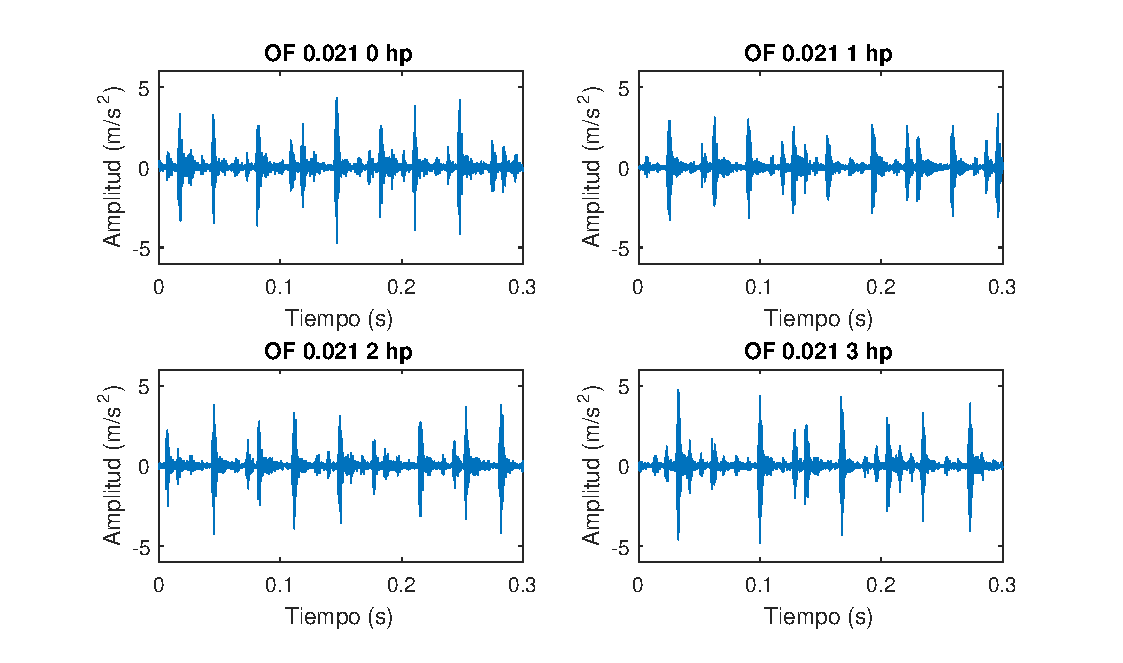
\includegraphics[scale=0.9]{./signalOF.eps}
  \caption{4 tipos de señal de vibración de un rodamiento, con una carga de 3 hp y 0,54 mm de diámetro de falla.}
  \label{fig:senales}
\end{figure}

\paragraph{}
La transformada rápida de Fourier (FFT) fue seleccionada como técnica de extracción de características por ser una herramienta de baja complejidad computacional y porque puede trasladar la señal original al dominio de la frecuencia. Sin embargo, tiene una serie de desventajas en este tipo de problemas en que la señal de vibración (Figura \ref{fig:senales}) es tremendamente compleja. Podríamos decir que la desventaja más importante es que, esta técnica es menos eficiente cuando las fallas son distribuidas y la señal tiene un comportamiento no lineal, el espectro de frecuencias varia en el tiempo y la técnica no es capaz de realzar las componentes impulsivas características de la falla.

\paragraph{}
En la Fig. \ref{fig:block} se encuentra el diagrama de flujo de los pasos descritos en esta sección, que van desde la carga de las señales, hasta el entrenamiento de la red neuronal profunda y las gráficas de las métricas para el diagnóstico. En el primer bloque del diagrama se encuentra la sucesión de pasos para obtener las características que alimentarán a la capa de entrada del clasificador.

\subsection{Deep learning}
\paragraph{}
En los años recientes, un nuevo enfoque de \textit{machine learning}, denominado \textit{deep learning}, ha llamado la atención de investigadores de múltiples áreas debido a una serie de ventajas respecto a otros enfoques. \textit{Deep learning} ha tenido un gran impacto en trabajos actuales de reconocimiento de voz, visión artificial y procesamiento del lenguaje natural, a causa de la efectividad empírica de este respecto a enfoques alternativos en estos ámbitos. El desarrollo de esta tecnología fue potenciado, en gran medida, por la creciente capacidad de cómputo de los equipos, y por el uso de los inmensos volúmenes de datos que son generados todos los días por la humanidad.

\paragraph{}
Esta ola de interés por el \textit{deep learning}, se centra principalmente en los perceptrón multicapa profundo (deep multilayer perceptron), las redes convolucionales profundas (deep convolutional network) y las redes neuronales recurrentes (recurrent neuronal network) \cite{mining}. Sin embargo, la mayoría de los métodos de \textit{deep learning} se basan en el perceptrón multicapa profundo, porque lo utilizan como el bloque esencial de construcción. Este nuevo enfoque formula el problema subyacente como una arquitectura en forma de red, en la que su capa de salida define una función de costos (también llamada función de perdida) que es necesaria para aprender.

\paragraph{}
El desarrollo del \textit{deep learning} está relacionado con el uso de técnicas de aprendizaje no supervisado como los diferentes tipos de autoencoder que existen para realizar un pre entrenamiento de las capas ocultas. De acuerdo a Ranzato et al. (2008) \cite{ranzato}, uno de los principales propósitos del aprendizaje no supervisado es producir buenas representaciones de los datos que puedan ser usadas para la detección, reconocimiento, predicción o visualización. Las buenas representaciones eliminan variaciones irrelevantes de los datos de entrada, mientras que se preserva la información que es útil para la tarea a realizar.

\paragraph{}
El aprendizaje no supervisado tiene la habilidad de crear jerarquías de características profundas (deep features hierarchies) mediante el apilado de módulos no supervisados uno encima de otro. Los módulos que se encuentran apilados se alimentan con los vectores de representación producidos por aquellos que se encuentran en un nivel inferior de la pila. Las representaciones producidas en el nivel superior captan las dependencias de alto nivel entre las variables de entrada, mejorando la capacidad de la red para capturar las regularidades subyacentes en los datos de entrada.

\subsubsection{Autoencoders}
\paragraph{}
Un autoencoder (AE) es una red neuronal artificial no supervisada de tres capas que es entrenada para replicar los datos de entrada en la salida. El entrenamiento de los AE es no supervisado en el sentido de que no requiere datos etiquetados para aprender a replicarlos en la salida. Este tipo especial de red neuronal es utilizada para pre entrenar las capas ocultas de las redes neuronales profundas, de manera que encuentran los mejores pesos sinápticos posibles que agilizan la búsqueda de mínimos globales para la función de costos. 

\begin{figure}[ht]
  \centering
    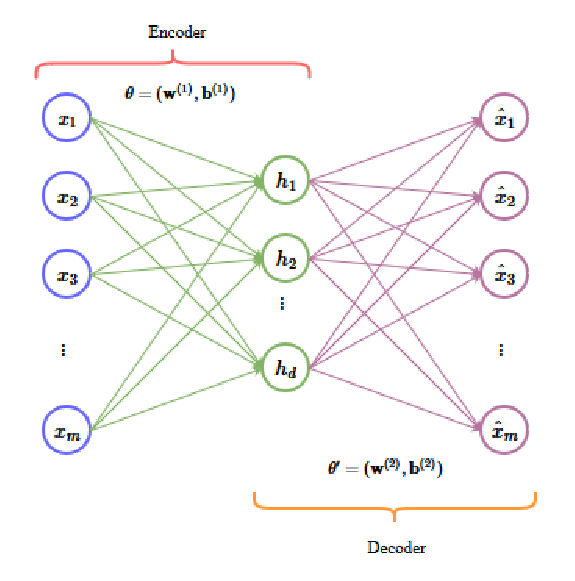
\includegraphics{./AE.eps}
  \caption{Diagrama que ilustra la estructura de un autoencoder formado por la red encoder (lado izquierdo) y la red decoder (lado derecho) con sus respectivos parámetros de entrenamiento.}
  \label{fig:ae}
\end{figure}

\paragraph{}
Es posible identificar dos estructuras en la red autoencoder, por una parte el codificador en el lado izquierdo de la Figura \ref{fig:ae}, que mapea los datos de entrada desde un espacio de alta dimensión en códigos de un espacio de baja dimensión. Por otra parte, que se encuentra al lado derecho de la Figura \ref{fig:ae}, reconstruye los datos de entrada a partir de los códigos obtenidos por la capa oculta llevándolos a su dimensión original \cite{shao}. Ahora que está claro cuál es el encoder y el decoder, podemos definir matemáticamente ambas estructuras.

\paragraph{}
Dadas las muestras de entrenamiento $\textbf{x}=(x_{1},x_{2},...,x_{n})$, donde la muestra $x_{n}\in \mathbb{R}^{m}$, se define la red encoder como una función codificadora $f_{\theta}$ (Ecc. \ref{f}) cuya tarea es representar estas muestras en un vector con códigos de menor dimensión denominado $\textbf{h}=(h_{1},h_{2},...,h_{n})$, en donde $h_{n} \in \mathbb{R}^{d}$ y $d<m$. La matriz de pesos sinápticos de la función encoder corresponde a $\textbf{w}^{(1)} = (w_{1}^{(1)},w_{2}^{(1)},...,w_{m}^{(1)})$ con $w_{m}^{(1)}\in \mathbb{R}^{d}$, mientras que $\textbf{b}^{(1)}=(b_{1}^{(1)},b_{2}^{(1)},...,b_{d}^{(1)})^T$ representa el arreglo de \textit{biases} pertenecientes a las neuronas de la capa oculta. Los pesos sinápticos y los \textit{biases} conforman $\theta$, el conjunto de parámetros a minimizar en la función de costos que será detallada más adelante.

\begin{equation}
\label{h}
\textbf{h}=f_{\theta}(\textbf{x})
\end{equation}

\begin{equation}
\label{f}
f_{\theta}(\textbf{x})=s_{f}(\textbf{w}^{(1)}\textbf{x}+\textbf{b}^{(1)})
\end{equation}

\begin{equation}
\label{teta1}
\theta=(\textbf{w}^{(1)},\textbf{b}^{(1)})
\end{equation}

\paragraph{}
La red decoder se define como una función de reconstrucción denotada como $g_{\theta'}$ (Ecc. \ref{g}), dicha función mapea el vector $\textbf{h}$ desde el espacio de baja dimensión en el que se encuentra, de vuelta al espacio de alta dimensión original realizando así la reconstrucción. Los datos reconstruidos se denotan mediante $\hat{\textbf{x}}=(\hat{x}_{1},\hat{x}_{2},...,\hat{x}_{n})$ (Ecc. \ref{xhat}), en donde $\hat{x}_{n}\in \mathbb{R}^{m}$. El primer parámetro que compone a $\theta'$ (Ecc. \ref{teta2}) perteneciente al decoder, es la matriz de pesos sinápticos de salida $\textbf{w}^{(2)} = (w_{1}^{(2)},w_{2}^{(2)},...,w_{m}^{(2)})$ con $w_{m}^{(2)}\in \mathbb{R}^{d}$. Mientras que el segundo, es el arreglo de \textit{biases} $\textbf{b}^{(2)}=(b_{1}^{(2)},b_{2}^{(2)},...,b_{d}^{(2)})^T$. 
\begin{equation}
\label{xhat}
\hat{\textbf{x}}=g_{\theta'}(\textbf{h})
\end{equation}

\begin{equation}
\label{g}
g_{\theta'}(\textbf{h})=s_{g}(\textbf{w}^{(2)}\textbf{h}+\textbf{b}^{(2)})
\end{equation}

\begin{equation}
\label{teta2}
\theta'=(\textbf{w}^{(2)},\textbf{b}^{(2)})
\end{equation}

\paragraph{}
Los conjuntos de parámetros $\theta$ y $\theta'$ de las redes encoder y decoder respectivamente, son aprendidos simultáneamente en la tarea de reconstruir en la mayor medida posible los datos originales de entrada. En otras palabras, es deseable obtener el menor error de reconstrucción (Ecc. \ref{xi}) posible a través de las $n$ muestras de entrenamiento, utilizando el error cuadrático medio (MSE). Este estimador es la función de costo estándar para los autoencoder y muchos otros algoritmos de \textit{machine learning} \cite{mining}.

\begin{equation}
\label{xi}
J_{mse}(\theta,\theta')=\frac{1}{2n}\sum_{i=1}^{n}{\|x_{i}-\hat{x}_{i}\|}^2
\end{equation}

\paragraph{}
El proceso de aprendizaje del autoencoder puede ser visto como un problema de optimización, porque tiene como objetivo encontrar valores que se aproximan al mínimo global de la función de costos. La función que debemos optimizar (Ecc. \ref{fcost}), también llamada función de pérdida, se compone por el error de reconstrucción (Ecc. \ref{xi}) y otro término llamado \textit{weight decay} (Ecc. \ref{weight}). De acuerdo a \cite{haykin}, el término \textit{weight decay} fuerza a algunos de los pesos sinápticos que tienen una pobre capacidad de generalización a tomar valores cercanos a 0,  evitando el sobreentrenamiento de la red.

\begin{equation}
\label{fcost}
\phi_{AE}(\theta,\theta')= J_{mse}(\theta,\theta') + J_{weight}(\theta,\theta')
\end{equation} 

\begin{equation}
\label{weight}
J_{weight}(\theta,\theta')=\frac{\lambda}{2}\sum_{l=1}^{2}\sum_{i=1}^{s_l}\sum_{j=1}^{s_{l+1}}({w^{(l)}_{ji}})^2 \quad s_{1}=m,s_{2}=d,s_{3}=m.
\end{equation}

\paragraph{}
Resulta común aplicar el algoritmo \textit{backpropagation}, ampliamente utilizado en \textit{machine learning}, de la función de costos de los autoencoder estándar para encontrar valores mínimos. Este algoritmo calcula el gradiente a la función de costos para encontrar direcciones, las cuales permiten actualizar los pesos y \textit{biases} iniciales, de manera que con cada iteración se acerquen más al mínimo global de la función. Obtenidos los mejores valores posibles, la capa oculta $\textbf{h}$ del autoencoder es capaz de representar a los datos de entrada en una dimensión menor que la original, sin perder información relevante para el reconocimiento de patrones.

\subsubsection{Sparse autoencoders}

\paragraph{}
Podemos definir al \textit{sparse} autoencoder, desde ahora denominado SAE, como una extensión del autoencoder estándar que obliga a sus unidades de la capa oculta a mantener una baja activación media. Creando así, características dispersas que logran una mejor generalización en la tarea de clasificar\cite{du}. El SAE impone un término de penalización (Ecc. \ref{spterm}) a las unidades de la capa oculta, forzando a que la activación media de cada unidad sea cercana al parámetro de dispersión $\rho$ que generalmente toma un valor muy pequeño cercano a 0. 

\begin{equation}
\label{sparse}
\phi_{SAE}(\theta,\theta')=\phi_{AE}(\theta,\theta')+J_{sparse}(\theta,\theta')
\end{equation}

La restricción se hace efectiva agregando el término de penalización a la función de costos del autoencoder estándar $\phi_{AE}$ (Ecc. \ref{fcost}), resultando en una nueva función de costos $\phi_{SAE}$ (Ecc. \ref{sparse}).

\begin{equation}
\label{spterm}
J_{sparse}(\theta,\theta')=\beta\sum_{j=1}^{d}KL(\rho||\hat{\rho_{j}})
\end{equation} 

\begin{equation}
\label{kl}
KL(\rho||\hat{\rho_{j}})={\rho} \log\frac{\rho}{\hat{\rho_{j}}}+(1-\rho)\log\frac{1-\rho}{1-\hat{\rho_{j}}}
\end{equation} 

\begin{equation}
\label{rho}
\hat{\rho_{j}}=\frac{1}{n}\sum_{k=1}^{n}h_{j,k}
\end{equation} 

\paragraph{}
$J_{sparse}$ impone la restricción de dispersión, $\beta$ controla el peso de esta restricción y $KL(\rho||\hat{\rho_{j}})$ (Ecc. \ref{kl}) es la divergencia Kullback-Leibler entre una variable aleatoria Bernoulli con media $\rho$ y una variable aleatoria Bernouilli media $\hat{\rho_{j}}$. La divergencia KL es una función estándar para medir la diferencia entre dos distribuciones de probabilidad diferentes. Definiremos $\hat{\rho_{j}}$ (Ecc. \ref{rho}) como la probabilidad media de activación en la j-ésima unidad de la capa oculta $\textbf{h}$ a través las $n$ muestras, y $\rho$ la probabilidad de activación deseada ($\rho\ll1$) \cite{song}. 

\paragraph{}
Una vez que hemos definido el término de dispersión y lo hemos incorporado a la función de costos del autoencoder (Ecc. \ref{scost}), aplicaremos el método del gradiente conjugado para actualizar los pesos y \textit{biases}. El método del gradiente conjugado pertenece a una clase de métodos de optimización de segundo orden conocidos colectivamente como métodos de dirección conjugada \cite{haykin}. La motivación para utilizar este método es que converge más rápido hacia un mínimo que el descenso del gradiente, y a la vez se evitan los requisitos de computación y almacenamiento del hessiano, como lo requiere el método de Newton.

\begin{equation}
\label{scost}
\phi_{SAE}(\theta,\theta')=\frac{1}{2n}\sum_{i=1}^{n}{\|x_{i}-\hat{x}_{i}\|}^2 + \frac{\lambda}{2}\sum_{l=1}^{2}\sum_{i=1}^{s_l}\sum_{j=1}^{s_{l+1}}({w^{(l)}_{ji}})^2 + \beta\sum_{j=1}^{d}KL(\rho||\hat{\rho_{j}})
\end{equation} 

Para simplificar la notación del método, definiremos $\Theta$ (Ecc. \ref{param}) como un arreglo que contiene los parámetros de la función de costos. Según la Ecc. \ref{gconjugado}, este método toma los parámetros iniciales y los actualiza sumándoles una dirección multiplicada por una tasa de aprendizaje denominada $\eta$. El arreglo que contiene las direcciones (Ecc. \ref{direcciones}) se obtiene utilizando la dirección previa multiplicada por el parámetro conjugado $\gamma$ más el residuo (Ecc. \ref{residuo}). El arreglo gradiente (Ecc. \ref{gradiente}) está compuesto por las derivadas parciales de la función de costos, a la vez que la derivada parcial $\frac{\partial{\phi_{SAE}}}{\partial{\theta}}$ se compone de las derivadas parciales de pesos y \textit{biases} (Ecc. \ref{parcial}).

\begin{equation}
\label{param}
\Theta = (\theta,\theta')
\end{equation} 

\begin{equation}
\label{gconjugado}
\Theta(n+1)=\Theta(n)+{\eta}s(n)
\end{equation}

\begin{equation}
\label{direcciones}
s(n+1)=r(n+1)+\gamma{s(n)}
\end{equation} 

\begin{equation}
\label{residuo}
r(n+1) = -\nabla{\phi_{SAE}(\Theta(n+1))}
\end{equation} 

\begin{equation}
\label{gradiente}
\nabla{\phi_{SAE}} = \left(\frac{\partial{\phi_{SAE}}}{\partial{\theta}},\frac{\partial{\phi_{SAE}}}{\partial{\theta'}}\right)
\end{equation}

\begin{equation}
\label{parcial}
\frac{\partial{\phi_{SAE}}}{\partial{\theta}} = \left(\frac{\partial{\phi_{SAE}}}{\partial{\textbf{w}^{(1)}}},\frac{\partial{\phi_{SAE}}}{\partial{\textbf{b}^{(1)}}}\right)
\end{equation}  
\subsection{Método de diagnóstico basado en DNN}
\label{sec:training}

\paragraph{}
En esta sección, se dará detalle del proceso de entrenamiento de la red neuronal profunda (DNN) y los elementos que la componen. La red utilizada en este modelo, posee una capa de entrada, dos capas ocultas y una capa de salida con la función de transferencia softmax. Las dos capas ocultas son pre entrenadas con dos \textit{sparse} autoencoder (SAE) respectivamente. Estas redes de tres capas permiten encontrar los parámetros de entrenamiento a la vez que reducen la dimensión de los datos de entrada codificandolos en un espacio de menor dimensión. 

\paragraph{}
Una vez que el primer SAE termina de aprender su representación de los datos a través del algoritmo del gradiente conjugado (Ecc. \ref{gradiente}), inicializa con sus parámetros óptimos $\theta_{1}$ a la primera capa oculta de la DNN como se muestra en la parte izquierda A de la Fig. \ref{fig:deepnet}. Luego el segundo SAE, constituido por la primera y la segunda capa oculta de la DNN, aprende un conjunto de parámetros que inicializa a la segunda capa oculta y los códigos de la segunda capa oculta alimentan a la regresión softmax para que sea entrenada.

\paragraph{}
Una vez obtenidos los parámetros de las capas ocultas, la DNN realiza un \textit{fine tuning} que básicamente es aplicar el algoritmo \textit{backpropagation} a la red entera para mejorar los pesos y \textit{biases} en conjunto. Se utiliza el descenso del gradiente en vez del gradiente conjugado porque los parámetros se encuentran cerca del mínimo global de la función de costos, por lo que no son necesarias demasiadas iteraciones en el proceso.

\begin{figure}[ht]
  \centering
    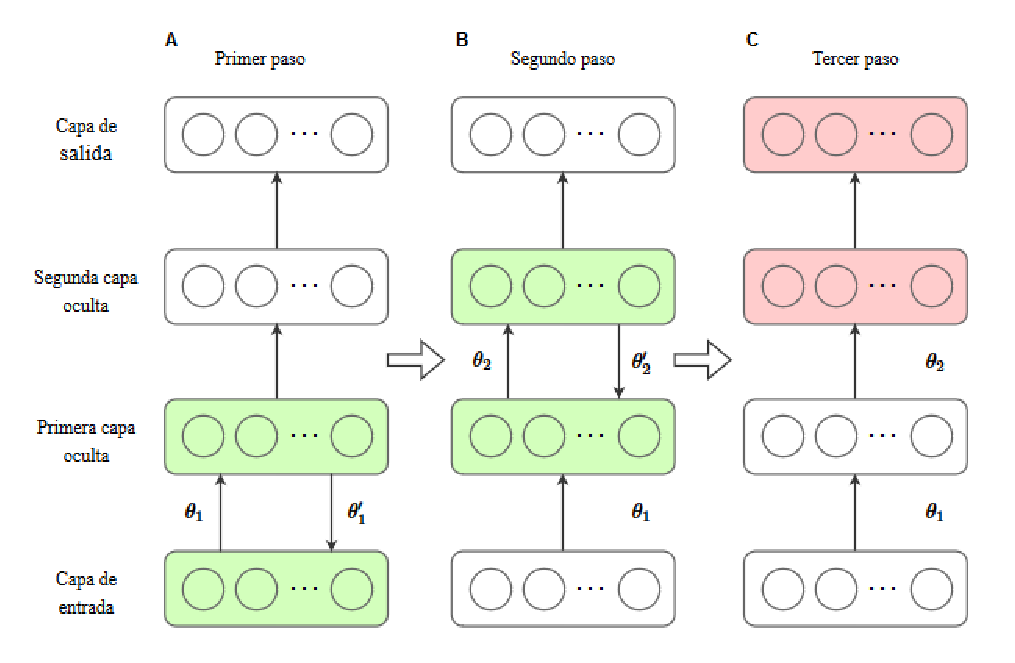
\includegraphics[scale=0.9]{./training.eps}
  \caption{Diagrama que representa el entrenamiento de los \textit{sparse} autoencoder y la asignación de sus parámetros a la DNN}
  \label{fig:deepnet}
\end{figure}

\section{Experimento y resultados}
\subsection{Origen de los datos}
\paragraph{}
Los datos utilizados en este trabajo corresponden a señales de vibración de un rodamiento de bolas, obtenidos de un experimento realizado por el Bearing Data Center of Case Western Reserve University \cite{case}. Los aparatos empleados en este laboratorio de vibraciones corresponden a: un motor de 2 hp a la izquierda del banco de pruebas (como se aprecia en la Figura \ref{fig:bearing}), un transductor/codificador de torque en el centro y un dinamómetro a la derecha. Un acelerómetro es el encargado de registrar las señales de vibración emitidas por el rodamiento que soporta el eje del motor.

\begin{figure}[ht]
  \centering
    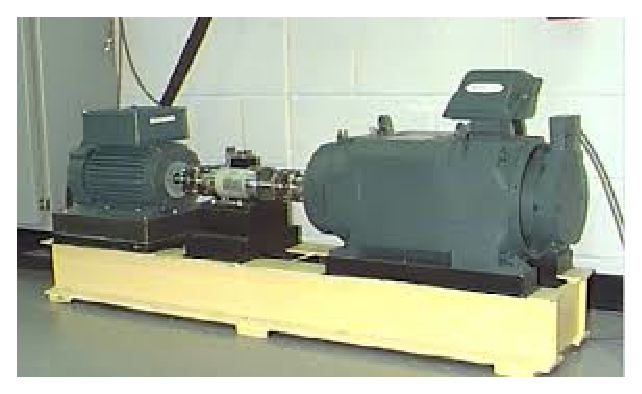
\includegraphics[scale=0.8]{./bearing.eps}
  \caption{Ilustración del experimento realizado por la Case Western Reserve University \cite{case}}
  \label{fig:bearing}
\end{figure}

\paragraph{}
El rodamiento ubicado en el \textit{drive end} fue sometido a descargas eléctricas que generaron defectos en un  punto único, con tres diámetros de falla: 0,007, 0,014 y 0,021 pulgadas. Estas imperfecciones son inducidas bajo las velocidades de rotación 1.730, 1.750 1.772 y 1.792 rpm y 4 diferentes cargas de 0, 1, 2 y 3 hp respectivamente. Por lo anterior es que los datos pueden ser organizados en conjuntos separados por velocidad/carga como se detallará en la siguiente sección. La frecuencia de muestreo es de 12 kHz para las cuatro condiciones de salud: normal (N), falla en el anillo externo (OF), falla en el anillo interno (IF) y falla en la bola (RF). 

\paragraph{}
El principal motivo para utilizar esta base de datos es que sirve como punto de comparación para este trabajo, permitiendo efectuar el contraste con investigaciones similares que realizan diagnóstico de fallas inteligente en rodamientos. De esta manera, es posible desarrollar conclusiones a cerca del desempeño de la configuración propuesta y de la aplicación del \textit{deep learning} a este tipo de problemas. Además, al tener tipos de fallas con severidades, es posible elevar el grado de complejidad del problema aparte de probar la capacidad de reconocimiento de más estados de salud con del modelo propuesto.

\subsection{Energía de los coeficientes de Fourier}
\label{sec:datasets}

\paragraph{}
Cinco conjuntos de datos, ilustrados en la Tabla \ref{table:tdatasets}, serán utilizados en este trabajo para probar el rendimiento del método propuesto. Los \textit{datasets} poseen 10 etiquetas de clasificación que corresponden a los 10 estados de salud del rodamiento, separados bajo las velocidades de eje de 1.797, 1.772, 1.750 y 1.720 rpm y las cargas 0, 1, 2 y 3 hp correspondientemente. El conjunto E es el de mayor tamaño, porque reúne las 4 velocidades y es, por lo tanto, el que más se aproxima a una señal de vibración de un rodamiento sometido a carga y velocidad variables.

\paragraph{}
El largo de la señal de vibración bruta es de 120.832 puntos, resultado de 10,06 segundos de medición y el tamaño de segmentación de las subseñales es de 2.048 puntos (unos 170,6 ms). Este tamaño de segmentación corresponde entre 5,12 a 4,9 veces el periodo de rotación, considerando que este fluctúa entre 400 y 418 puntos de la señal. Con dicho tamaño de segmentación, tal como lo indica la Tabla \ref{table:tdatasets}, la cantidad de muestras totales que tienen los 4 primeros \textit{datasets} es de 590 y 2.360 en el caso del E.

\begin{table}
\scalebox{0.9}{
\begin{tabular}{c c c c c c}
\toprule
Dataset & Carga (hp) & Cantidad de muestras & Tipo de falla & Diámetro de falla (in) & Etiqueta\\
\midrule
A/B/C/D/E & 0/1/2/3/0-3 & 59/59/59/59/236 & RF & 0,007 & 1\\
\addlinespace
& & 59/59/59/59/236 & RF & 0,014 & 2\\
\addlinespace
& & 59/59/59/59/236 & RF & 0,021 & 3\\
\addlinespace
& & 59/59/59/59/236 & IF & 0,007 & 4\\
\addlinespace
& & 59/59/59/59/236 & IF & 0,014 & 5\\
\addlinespace
& & 59/59/59/59/236 & IF & 0,021 & 6\\
\addlinespace
& & 59/59/59/59/236 & OF & 0,007 & 7\\
\addlinespace
& & 59/59/59/59/236 & OF & 0,014 & 8\\
\addlinespace
& & 59/59/59/59/236 & OF & 0,021 & 9\\
\addlinespace
& & 59/59/59/59/236 & N & N/A & 10\\
\bottomrule
\end{tabular}}
\caption{Descripción de los 5 \textit{datasets}.}
\label{table:tdatasets}
\end{table}

\paragraph{}
Luego de obtener las subseñales de 2.048 puntos, se les aplica la transformada rápida de Fourier (FFT) obteniendo la misma cantidad de componentes de frecuencia. Dado que la transformada tiene la propiedad de simetría, es posible tomar los primeros 1.024 coeficientes de Fourier para cada muestra. A continuación, se les aplica valor absoluto y se elevan al cuadrado, adquiriendo el espectro energético de las subseñales.

\subsection{Proceso de entrenamiento y testing}
\paragraph{}
Obtenida la energía de los coeficientes de Fourier, se reordenan de manera aleatoria las nuevas muestras contenidas en los conjuntos de datos y se divide cada uno estos en dos partes: un conjunto de entrenamiento con 413 muestras (70\%) y uno de \textit{testing} con 177 muestras (30\%). El conjunto de entrenamiento tiene como objetivo encontrar los mejores parámetros posibles de las capas ocultas de la DNN (pesos y \textit{biases}). El de \textit{testing} es usado para medir la exactitud (Ecc. \ref{acc}) del modelo propuesto en este trabajo.

\begin{equation}
\label{precision}
Precisi\acute{o}n = \frac{TP}{TP+FP}
\end{equation}

\begin{equation}
\label{sensibilidad}
Sensibilidad = \frac{TP}{TP+FN}
\end{equation}

\begin{equation}
\label{fscore}
F_{1}score = \frac{2\cdot{Precisi\acute{o}n}\cdot{Sensibilidad}}{Precisi\acute{o}n\cdot{Sensibilidad}}
\end{equation}

\begin{equation}
\label{acc}
Exactitud = \frac{VP+VN}{VP+FP+VN+FN}
\end{equation} 

\paragraph{}
Además de la exactitud, se emplean métricas que son habitualmente usadas en problemas de clasificación multiclase. Resulta común usar la validación cruzada para evaluar el aprendizaje de técnicas de inteligencia artificial, sin embargo, en este trabajo solo se corren 30 ejecuciones aleatorias por \textit{dataset} sin este método de prueba. A los resultados de estas 30 pruebas, se les calcula la exactitud media, la exactitud promedio por clase, el $F_{1}$score (Ecc. \ref{fscore}) o media armónica por clase y el $F_{1}$score medio.

\paragraph{}
La DNN diseñada está compuesta por 4 capas, el número de unidades de la primera es 1.024, mientras que el de la cuarta capa es de 10, equivalente a la cantidad de clases. La segunda y la tercera corresponden a las capas ocultas, cuyas cantidades óptimas de nodos es complejo de encontrar, por lo que en este trabajo fueron determinadas a través de prueba y error. Las mejores cantidades de nodos ocultos encontradas son: 105 (aproximadamente un décimo de los nodos de la capa de entrada) y 25 (aproximadamente un cuarto de la primera capa oculta) unidades.

\begin{table}
\centering
\scalebox{0.9}{
\begin{tabular}[c]{c c c c c c c c}
\toprule
Nro. & $\lambda_{1}$ & $\beta_{1}$ & $\rho_{1}$ & $\lambda_{2}$ & $\beta_{2}$ & $\rho_{2}$ & Exactitud (\%)\\
\midrule
1 & 0,0179 & 0,9226 & 0,2623 & 0,0155 & 0,9450 & 0,1104 & 99,7363 $\pm$ 0,3723\\
\addlinespace
2 & 0,0199 & 0,9876 & 0,0143 & 0,0008 & 0,9405 & 0,2718 & 99,9294 $\pm$ 0,0964\\
\addlinespace
3 & 0,0029 & 0,9865 & 0,3396 & 0,0062 & 0,9712 & 0,2620 & 99,9718 $\pm$ 0,0938\\
\addlinespace
4 & 0,0201 & 0,9488 & 0,3735 & 0,0012 & 0,9736 & 0,0650 & 99,9153 $\pm$ 0,1263\\
\addlinespace
5 & 0,0139 & 0,9740 & 0,2715 & 0,0023 & 0,9249 & 0,0476 & 99,9153 $\pm$ 0,1088\\
\addlinespace
6 & 0,0023 & 0,9213 & 0,3031 & 0,0181 & 0,9491 & 0,1993 & 99,8729 $\pm$ 0,1868\\
\addlinespace
7 & 0,0062 & 0,9437 & 0,2972 & 0,0153 & 0,9456 & 0,3838 & 99,9859 $\pm$ 0,0431\\
\addlinespace
8 & 0,0121 & 0,9832 & 0,1569 & 0,0071 & 0,9617 & 0,1361 & 99,9670 $\pm$ 0,0712\\
\addlinespace
9 & 0,0210 & 0,9733 & 0,2621 & 0,0209 & 0,9667 & 0,2341 & 99,8635 $\pm$ 0,2178\\
\addlinespace
10 & 0,0212 & 0,9867 & 0,0684 & 0,0009 & 0,9703 & 0,0895 & 99,9718 $\pm$ 0,0684\\
\bottomrule
\end{tabular}}
\caption{10 conjuntos de hiperparámetros probados con 30 ejecuciones en el dataset E, el formato de la exactitud es: Exactitud media $\pm$ desviación estándar.}
\label{table:parameters}
\end{table}

\paragraph{}
Durante el proceso de entrenamiento del primer SAE, los pesos y \textit{biases} son iniciados de manera aleatoria, mientras que los del segundo SAE son inicializados con los mejores parámetros del primero. La función de transferencia de los nodos de la capa oculta de los SAE es la logística sigmoide y la cantidad de iteraciones en el proceso de entrenamiento es de 200. Por su parte, la capa de salida tiene una función softmax y su cantidad de iteraciones en el entrenamiento es el mismo valor mencionado en el SAE. 

\paragraph{}
Los hiperparámetros penalizador de pesos ($\lambda$), penalizador de dispersión ($\beta$) y proporción de dispersión ($\rho$) de los \textit{sparse} autoencoder son complejos de hallar, convirtiendo la búsqueda manual de estos en una tarea difícil. Para encontrar los mejores hiperparámetros, fue necesario construir una grilla con valores aleatorios normalmente distribuidos para los dos SAE y probar el desempeño de estos. La Tabla \ref{table:parameters} muestra las 10 agrupaciones con valores que fueron probados en la DNN con el \textit{dataset} E, y también los resultados de cada agrupación luego de 30 ejecuciones.

\paragraph{}
Los intervalos para construir la grilla de la Tabla \ref{table:parameters} son los siguientes: [0,0002;0,022], [0,91;0,99] y [0,00002;0,4] para $\lambda$, $\beta$ y $\rho$ respectivamente. Como es posible observar en aquella Tabla, ninguna agrupación de valores obtuvo una exactitud media menor a 99,86\% y la mayoría registró una baja desviación estándar. Como consecuencia de esto, es posible afirmar que la variación de los valores para estos hiperparámetros, dentro los intervalos presentados, no genera grandes diferencias en los resultados.

\paragraph{}
La séptima agrupación de valores obtuvo la mayor exactitud promedio y la menor desviación estándar, lo que hace pensar que son los mejores candidatos por homogeneidad de resultados y exactitud. Estos valores son empleados para entrenar el modelo con los 5 \textit{datasets}, obteniendo así los resultados de 30 procesos de entrenamiento y \textit{testing} para cada uno de ellos. Dichos resultados se encuentran en la Tabla \ref{table:results}, incluyendo también la exactitud mínima y máxima alcanzada por el modelo en cada \textit{dataset}.

\begin{table}
\centering
\scalebox{0.9}{
\begin{tabular}[c]{c c c c c c c}
\toprule
Dataset & Carga (hp) & Exactitud m. (\%) & D. estándar & Mínimo (\%) & Máximo (\%) & Tiempo e. (s)\\
\midrule
A & 0 & 99,8117 & 0,3089 & 98,8701 & 100 & 64,860\\
\addlinespace
B & 1 & 99,9623 & 0,1433 & 99,4350 & 100 & 59,106\\
\addlinespace
C & 2 & 99,9829 & 0,0936 & 99,4872 & 100 & 62,127\\
\addlinespace
D & 3 & 99,9058 & 0,2142 & 99,4350 & 100 & 64,101\\
\addlinespace
E & 0-3 & 99,9718 & 0,0862 & 99,5763 & 100 & 196,268\\
\bottomrule
\end{tabular}}
\caption{Resultados del diagnóstico de cada \textit{dataset}.}
\label{table:results}
\end{table}

\paragraph{}
Como es posible observar en la Tabla \ref{table:results}, la exactitud promedio supera el 99,80\% en todos los \textit{datasets} y todos alcanzan el 100\% en la mayoría de las ejecuciones. El \textit{dataset} A es el que menor homogeneidad presenta en sus resultados, con 21 oportunidades en las que alcanzó el 100\%. El resto de los \textit{datasets} sobrepasa el 99,90\% de exactitud promedio y sus resultados son bastante homogéneos, sobretodo en el C y el E.

\paragraph{}
Si se presta atención a los resultados del \textit{dataset} E en las Tablas \ref{table:parameters} y \ref{table:results}, se puede apreciar la exactitud media cambia desde un 99,9859\% a un 99,9718\%. Este cambio se debe a que los valores de los pesos y \textit{biases} se inician de manera aleatoria en el primer SAE, haciendo variar la exactitud de cada ejecución. Este efecto de variación influye en todas las pruebas de todos los \textit{datasets} y es responsable en parte, de la heterogeneidad de los resultados del diagnóstico.

\paragraph{}
En la Figura \ref{fig:accge} es posible distinguir que en 30 procesos de entrenamiento y \textit{testing}, el modelo alcanza el 100\% de exactitud en 26 oportunidades (86,6\%). De aquellas ejecuciones en las que no se consigue el 100\%, la mas baja es de un 99,5763\%, la cual provoca un impacto en la exactitud media y en la desviación estándar. Sin embargo, las 4 caídas (13,4\%) en la exactitud son de menor magnitud respecto a las bajas que presentan los demás \textit{dataset}, lo cual se puede percibir en la Figura \ref{fig:exg}.

\paragraph{}
Respecto a los resultados del diagnóstico de los 5 \textit{datasets}, la Figura \ref{fig:exg} presenta las curvas de exactitud a través de las ejecuciones. La Figura deja en evidencia que las caídas de exactitud en los \textit{datasets} con excepción del A, están en torno del 99,4\%, lo que sugiere que los resultados fueron bastante parecidos y que no hay una gran variabilidad. De no ser por la baja de exactitud del \textit{dataset} E en la ejecución número 14, los resultados serían aun más parejos.

\paragraph{}
La exactitud por etiqueta de clasificación se encuentra contemplada en la Figura \ref{fig:accge}, la cual nos advierte que el modelo propuesto tiene problemas en ciertas clases. Aquellas son las 1, 2 y 3 correspondientes a fallas en las bolas del rodamiento (0,007, 0,014 y 0,021 pulgadas respectivamente), clases que registran sus rendimientos más bajos en el \textit{dataset} A. En este \textit{dataset} el rodamiento no soporta una carga, haciendo que la señal que se genera con el contacto de la falla con otras superficies sea tenue, complicando la tarea de clasificación.

\paragraph{}
La gráfica del F-score (o media armónica) de las 5 pruebas, materializada en la Figura \ref{fig:fscG}, es bastante parecida a la de la exactitud media, solo que las bajas de exactitud son más acentuadas. En la Figura \ref{fig:fsc} se encuentra el F-score por etiqueta obtenido de las pruebas, en ella se da cuenta de las grandes caídas de exactitud de los \textit{dataset} A y D. Ambas Figuras son parecidas a las de exactitud promedio y por etiqueta, con la diferencia que se ven con mayor énfasis las bajas de exactitud. 


\begin{figure}[ht]
  \centering
    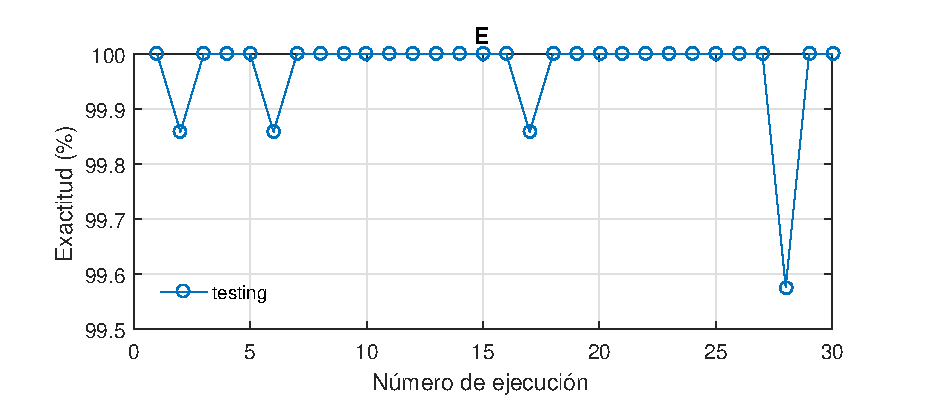
\includegraphics[scale=0.9]{./AccGE.eps}
  \caption{Resultados del diagnóstico en 30 \textit{trials} del \textit{dataset} E.}
  \label{fig:accge}
\end{figure}

\begin{figure}[ht]
  \centering
    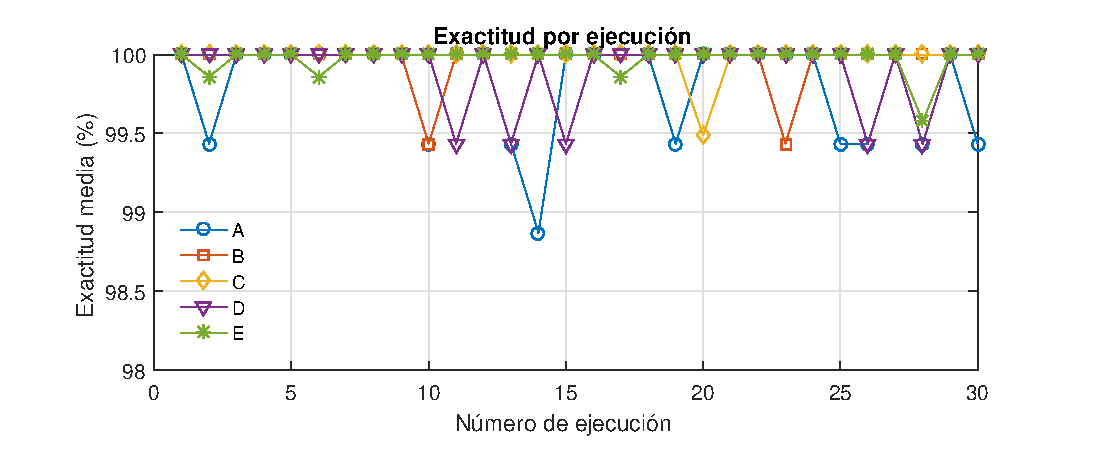
\includegraphics[scale=0.9]{./AccG.eps}
  \caption{Exactitud promedio del diagnóstico en 30 \textit{trials} de los 5 \textit{datasets}.}
  \label{fig:exg}
\end{figure}

\begin{figure}[ht]
  \centering
    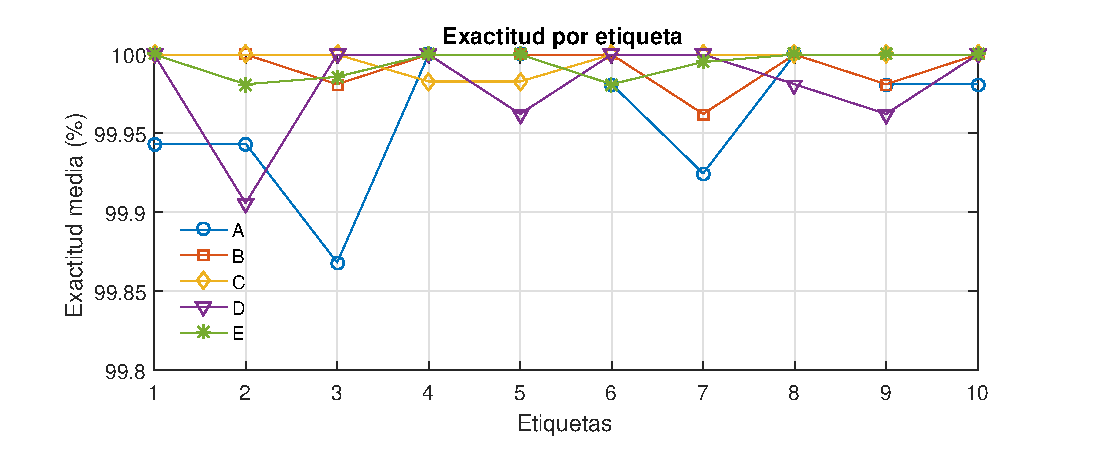
\includegraphics[scale=0.9]{./Acc.eps}
  \caption{Exactitud por clase en 30 \textit{trials} de los 5 \textit{datasets}.}
  \label{fig:exact}
\end{figure}

\begin{figure}[ht]
  \centering
    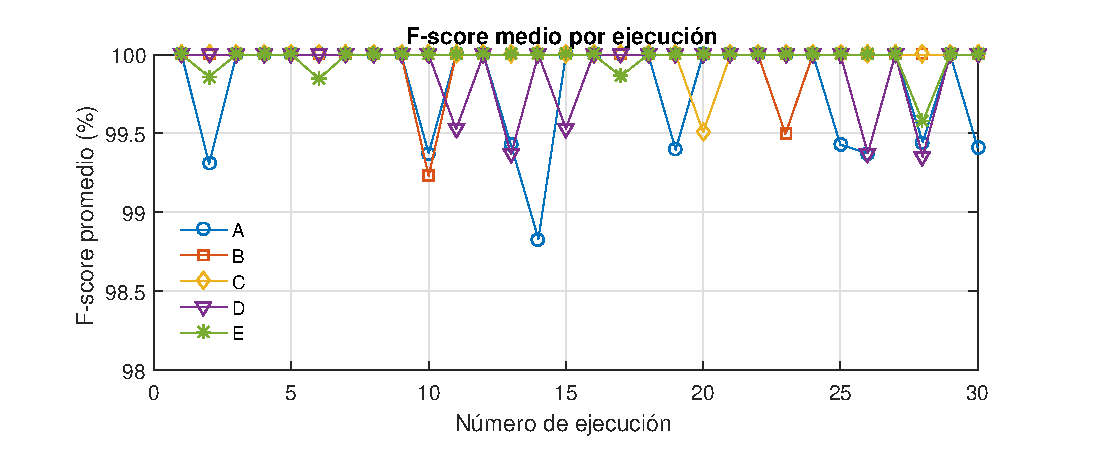
\includegraphics[scale=0.9]{./FscG.eps}
  \caption{F-score en 30 \textit{trials} de los 5 \textit{datasets}.}
  \label{fig:fscG}
\end{figure}

\begin{figure}[ht]
  \centering
    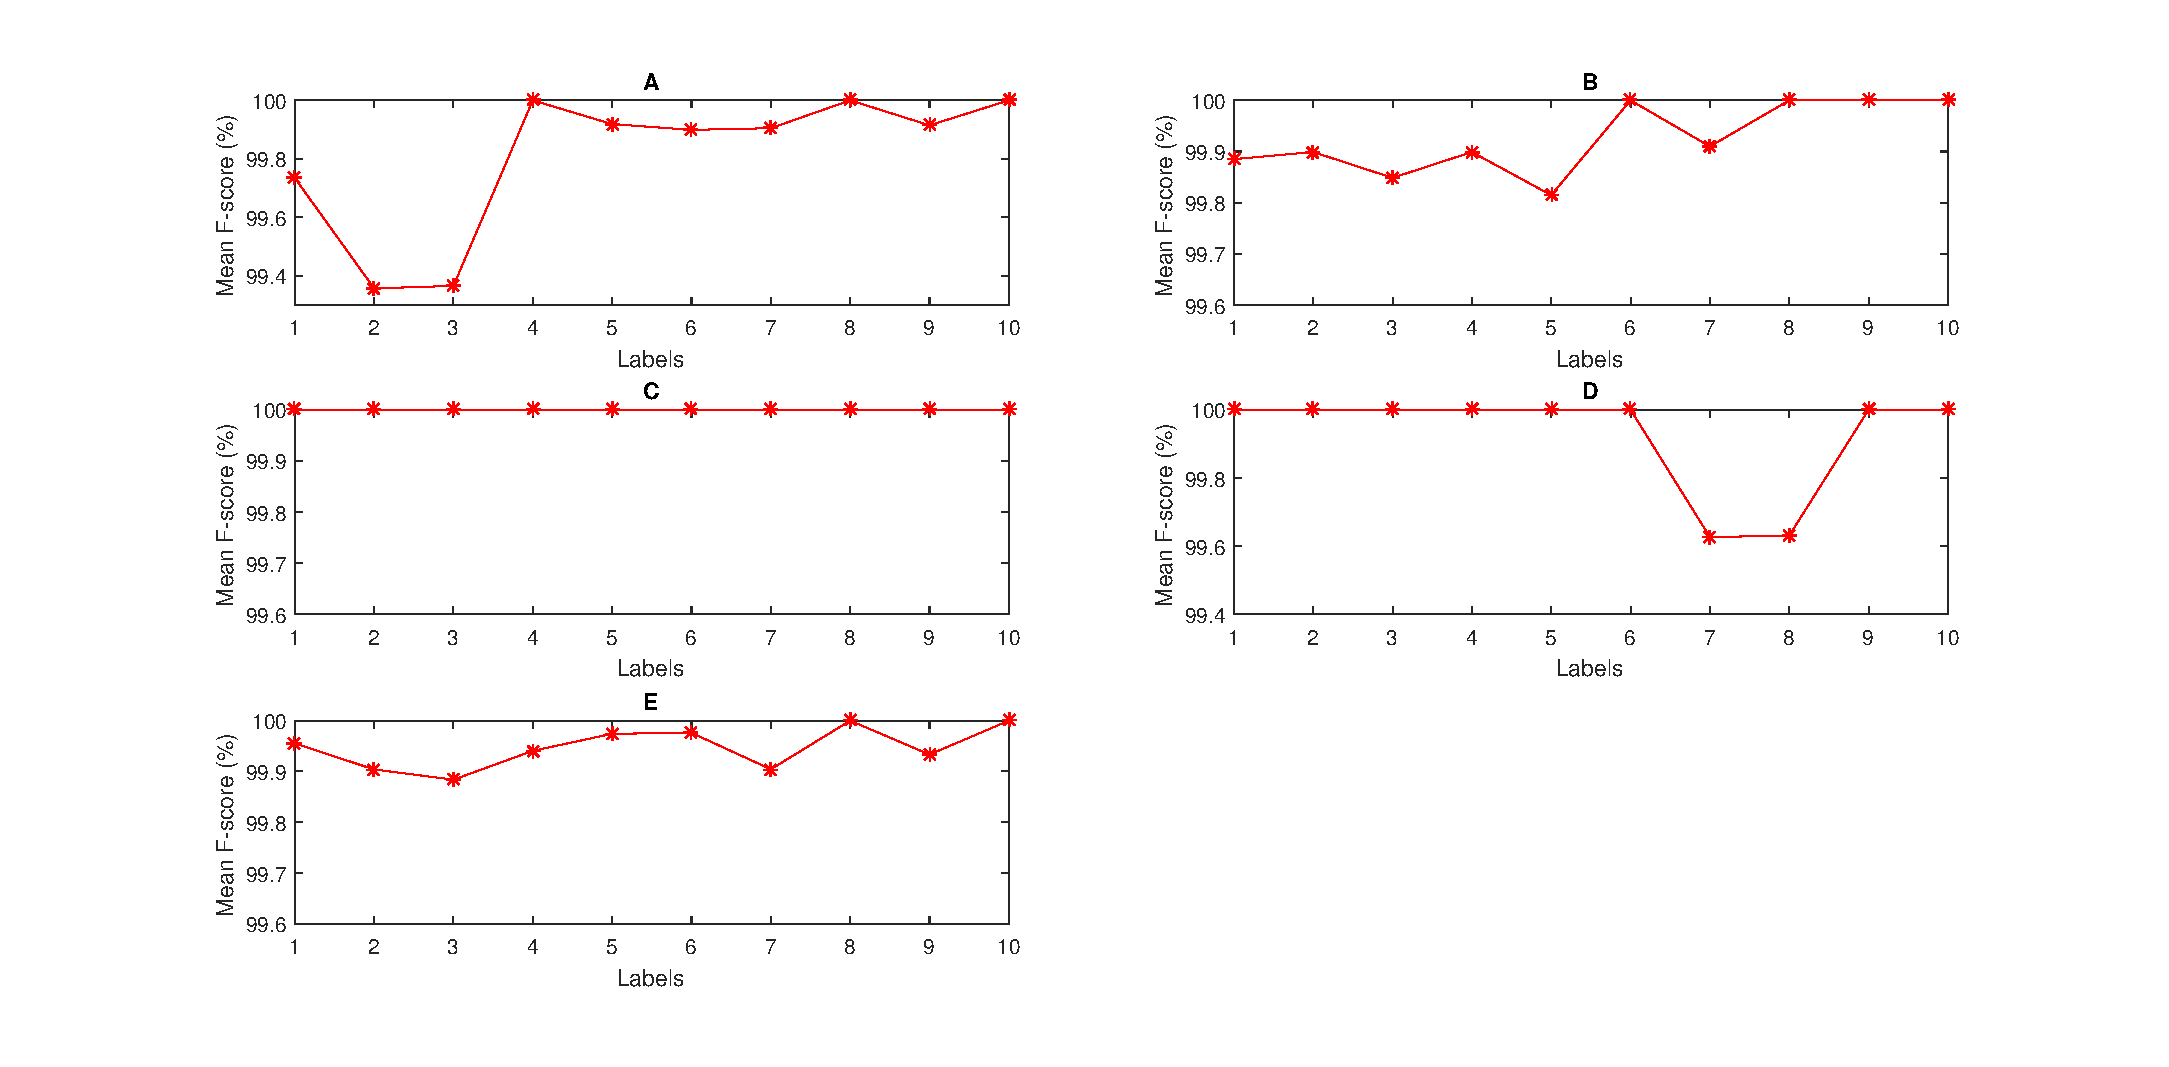
\includegraphics[scale=0.9]{./Fsc.eps}
  \caption{F-score por clase en 30 \textit{trials} de los 5 \textit{datasets}.}
  \label{fig:fsc}
\end{figure}

\paragraph{}
Con el objetivo de medir la eficiencia del modelo propuesto en este trabajo, se hará la comparación de los resultados obtenidos con dos investigaciones, Rodríguez et al. (2017) \cite{nibaldo} y Jia et al. (2016) \cite{jia} . El primer autor postula un método de diagnóstico inteligente empleando la transformada wavelet estacionaria, la descomposición en valores singulares de los coeficientes wavelet y una máquina de aprendizaje extremo. El segundo propone un método con la amplitud de los coeficientes de Fourier y una DNN con 3 autoencoders apilados.

\paragraph{}
Como pudimos observar en los párrafos anteriores, el método propuesto alcanza una exactitud promedio del 99,97\% en 30 ejecuciones o \textit{trials}, y una desviación estándar de 0,0862. Mientras que el método postulado por el autor Rodríguez et al. (2017) \cite{nibaldo}, logra una exactitud del 100\% en 50 \textit{trials} con una desviación estándar muy baja equivalente al 0,008. Esta comparación es en base a los resultados del \textit{dataset} E y deja claro que el \textit{deep learning} presenta desventajas frente a un modelo con técnicas de extracción de características más elaboradas y un clasificador con menos capas ocultas.

\paragraph{}
Las principales desventajas del modelo propuesto frente a este primer autor, es que no logra igualar la calidad de diagnóstico y la estabilidad de los resultados. La técnica de \textit{deep learning} aplicada en este trabajo requiere grandes tiempos de entrenamiento, mucho mayores que los de la maquina de aprendizaje extremo, y aun así tiene peores resultados. Además, la DNN requiere seleccionar una mayor cantidad de hiperparámetros, los cuales demostraron tener un comportamiento no lineal con respecto a la exactitud del diagnóstico, acrecentando la dificultad de hallar buenos valores para ellos.  

\paragraph{}
El segundo autor Jia et al. (2016) \cite{jia}, 


\begin{figure}[ht]
  \centering
    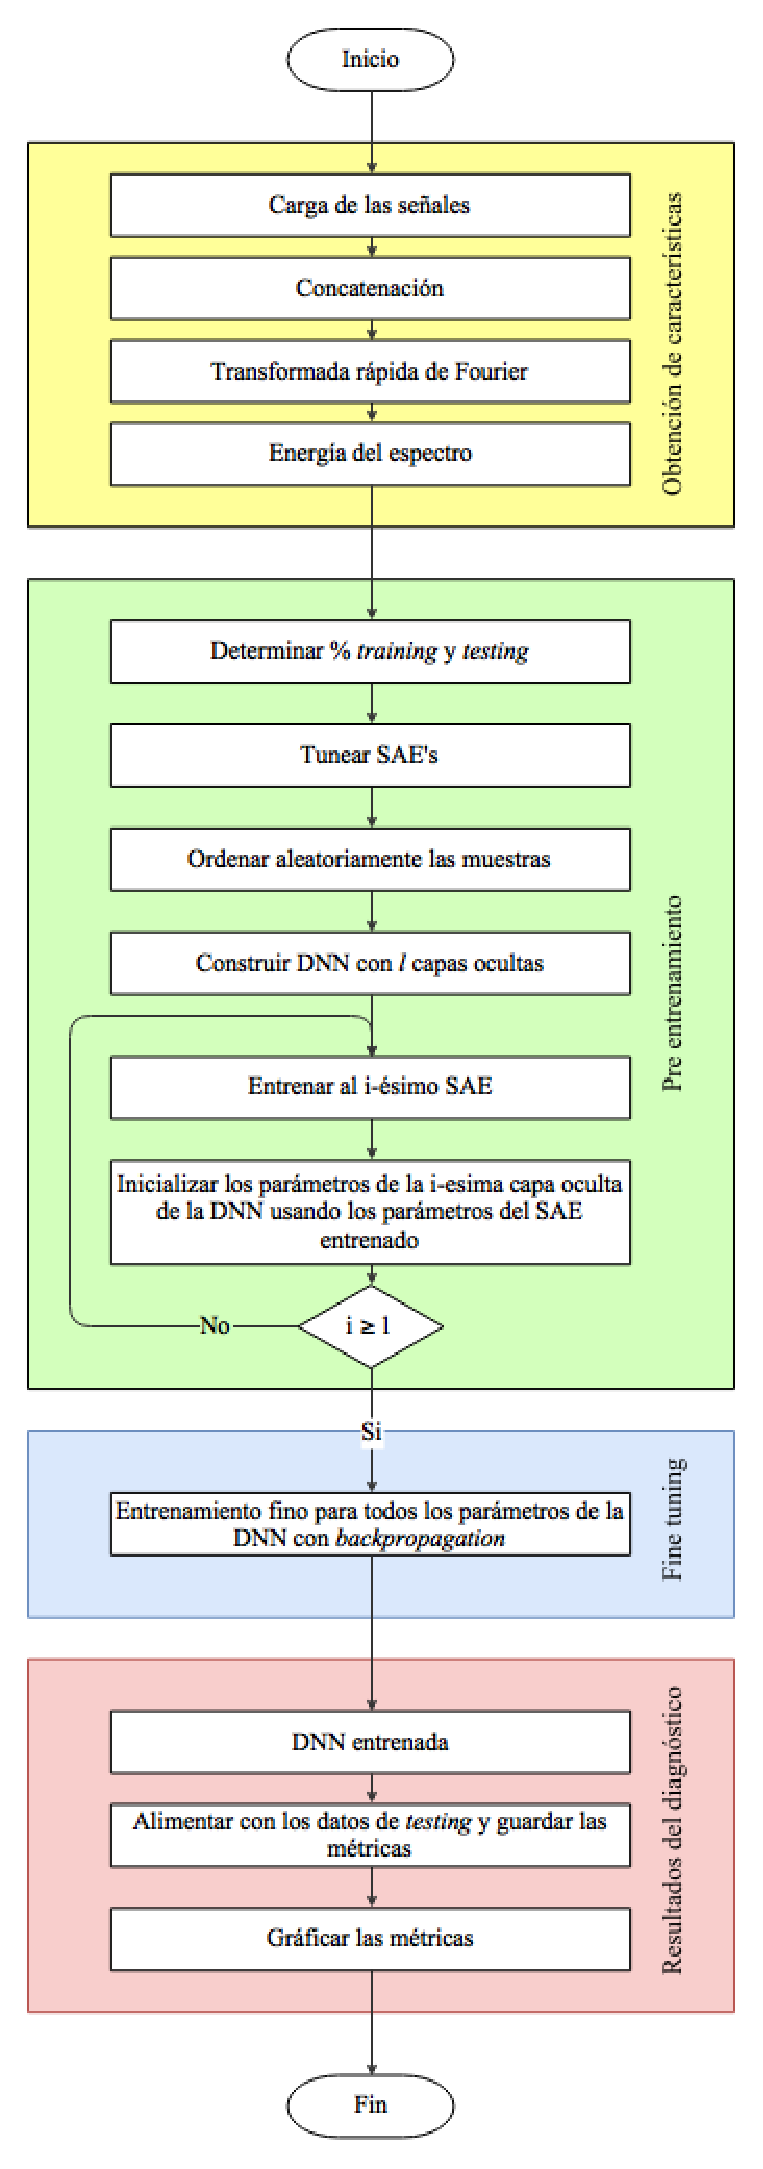
\includegraphics[scale=0.6]{./block.eps}
  \caption{Diagrama de flujo de los procesos que se llevan a cabo para entrenar y probar el modelo propuesto.}
  \label{fig:block}
\end{figure}

\section{Conclusión}
\paragraph{}
Como conclusión, 



\clearpage

\begin{thebibliography}{9}
\bibitem{seeraa} Manjeevan Seeraa, M.L. Dennis Wonga \& Asoke K. Nandic (2017). Classification of ball bearing faults using a hybrid intelligent model. \textit{Applied Soft Computing}, \textit{57}, 427–435.

\bibitem{zhan} Yimin Zhan \& Chris K. Mechefske (2007). Robust detection of gearbox deterioration using compromised
autoregressive modeling and Kolmogorov–Smirnov test statistic—Part I: Compromised autoregressive modeling with the
aid of hypothesis tests and simulation analysis. \textit{Mechanical Systems and Signal Processing}, \textit{21}, 1953–1982.

\bibitem{issam} Issam Attoui, Nadir Fergani, Nadir Boutasseta, Brahim Oudjani \& Adel Deliou (2017). A new time–frequency method for identification and classification of ball bearing faults. \textit{Journal of Sound and Vibration}, \textit{397}, 241-265.

\bibitem{fu} Yunxiao Fu, Limin Jia, Yong Qin \& Jie Yang (2016). Product Function Correntropy and Its Application in Rolling bearing Fault Identification. \textit{Measurement}, 88-99.

\bibitem{li} Wei Li, Zhencai Zhu, Fan Jiang, Gongbo Zhou \& Guoan Chen (2015). Fault diagnosis of rotating machinery with a novel statistical feature extraction and evaluation method. \textit{Mechanical Systems and Signal Processing}, \textit{50-51}, 414-426.

\bibitem{guo} Hong Guo, Lindsay B. Jack \& Asoke K. Nandi (2005). Feature Generation Using Genetic Programming With Application to Fault Classification. \textit{IEEE Transactions on Systems, Man, and Cybernetics, Part B (Cybernetics)}, \textit{35}(1), 89-99.

\bibitem{zhu} Xiaoran Zhu, Youyun Zhang \& Yongsheng Zhu (2012). Intelligent fault diagnosis of rolling bearing based on kernel neighborhood rough sets and statistical features. \textit{Journal of Mechanical Science and Technology}, \textit{26}(9), 2649-2657.

\bibitem{jia} Feng Jia, YaguoLei, Jing Lin, Xin Zhou \& Na Lu (2015). Deep neural networks: A promising tool for fault characteristic mining and intelligent diagnosis of rotating machinery with massive data. \textit{Mechanical Systems and Signal Processing}, \textit{72-73}, 303-315.

\bibitem{yu} Yang Yu, YuDejie \& Cheng Junsheng (2006). A roller bearing fault diagnosis method based
on EMD energy entropy and ANN. \textit{Journal of Sound and Vibration}, \textit{294}, 269–277. 

\bibitem{chang} Changting Wang \& Robert X. Gao (2002). Wavelet Transform with Spectral Post-Processing for
Enhanced Feature Extraction. \textit{IEEE Instrumentation and Measurement Technology Conference}, \textit{52}(4), 1296-1301.

\bibitem{ran} Ran Zhang, Zhen Peng, Lifeng Wu, Beibei Yao \& Yong Guan (2017). Fault Diagnosis from Raw Sensor Data Using Deep Neural Networks Considering Temporal Coherence. \textit{Sensors}, \textit{17}(3), 549-566.

\bibitem{ali} Jaouher Ben Ali, Nader Fnaiech, Lotfi Saidi, Brigitte Chebel-Morello \& Farhat Fnaiech (2015). Application of empirical mode decomposition and artificial neural network for automatic bearing fault diagnosis based on vibration signals. \textit{Applied Acoustics}, \textit{89}, 16–27.

\bibitem{wu} Lifeng Wu, Beibei Yao, Zhen Peng \& Yong Guan (2017). Fault Diagnosis of Roller Bearings Based on a Wavelet Neural Network and Manifold Learning. \textit{Applied Science}, \textit{7}, 158-168. 

\bibitem{rai} V.K. Rai \& A.R. Mohanty (2007). Bearing fault diagnosis using FFT of intrinsic mode functions in Hilbert–Huang transform. \textit{Mechanical Systems and Signal Processing}, \textit{21}, 2607–2615.

\bibitem{anthony} Wheeler, Anthony J. \& Ganji, Ahmad R. (2009). \textit{Introduction to Engineering Experimentation} (3rd ed., pp. 107-117). New Jersey: Prentice Hall.

\bibitem{robert} Gray, Robert M. \& Goodman, Joseph W. (1995). \textit{Fourier Transforms: An Introduction for Engineers} (1st ed., pp. 53-57). New York: Springer.

\bibitem{shao} Shao Haidong, Jiang Hongkai, Zhao Huiwei \& Wang Fuan (2017). A novel deep autoencoder feature learning method for rotating machinery fault diagnosis. \textit{Mechanical Systems and Signal Processing}, \textit{95}, 187-204. 

\bibitem{song} Song-Zhi Su, Zhi-Hui Liu, Su-Ping Xu, Shao-Zi Li \& Rongrong Ji (2014). Sparse auto-encoder based feature learning for humanbody detection in depth image. \textit{Signal Processing}, \textit{112}, 43-52.

\bibitem{yufeng} Yufeng Zhang, Zhenyu Guo, Weilian Wang, Side He, Ting Lee \& Murray Loew (2003). A comparison of the wavelet and short-time fourier transforms for Doppler spectral analysis. \textit{Medical Engineering \& Physics}, \textit{25}, 547-557.

\bibitem{aure} Aurelien Prudhom, Jose Antonino-Daviu, Hubert Razik \& Vicente Climente-Alarcon (2015). Time-frequency vibration analysis for the detection of motor damages caused by bearing currents. \textit{Mechanical Systems and Signal Processing}, \textit{84}, 747-762.

\bibitem{chen} Zhiqiang Chen, Shengcai Deng, Xudong Chen, Chuan Li, René-Vinicio Sanchez \& Huafeng Qin (2017). Deep neural networks-based rolling bearing fault diagnosis. \textit{Microelectronics Reliability}, \textit{75}, 327-333.

\bibitem{konar} P. Konar \& P. Chattopadhyay (2011). Bearing fault detection of induction motor using wavelet and Support Vector Machines (SVMs). \textit{Applied Soft Computing}, \textit{11}, 4203-4211.

\bibitem{mao} Wentao Mao, Jianliang He, Yuan Li \& Yunju Yan (2017). Bearing fault diagnosis with auto-encoder extreme learning machine: A comparative study. \textit{Proceedings of the Institution of Mechanical Engineers, Part C: Journal of Mechanical Engineering Science}, \textit{231}(8), 1560-1578.

\bibitem{kanpaj} Kanpaj Gupta \& M.K. Pradhan (2017). Fault detection analysis in rolling element bearing: A review, \textit{Materials Today: Proceedings}, \textit{4}, 2085-2094.

\bibitem{mining} Witten, Ian H. \& Frank, Eibe \& Hall, Mark A. \& Pal, Christopher J. (2016). \textit{Data Mining: Practical Machine Learning Tools and Techniques-Morgan Kaufmann} (4th ed., pp. ), Morgan Kaufmann.

\bibitem{haykin} Haykin, Simon. (2009). \textit{Neural Networks and Learning Machines} (3rd ed., pp.), Pearson.

\bibitem{ranzato} Marc’Aurelio Ranzato, Y-Lan Boureau \& Yann LeCun (2008). Sparse feature learning for deep belief networks. \textit{Advances in Neural Information Processing Systems}, \textit{20}, 1185–1192.

\bibitem{du} Erzhu Li, Peijun Du, Alim Samat, Member, Yaping Meng \& Meiqin Che (2017). Mid-Level Feature Representation via Sparse Autoencoder for Remotely Sensed Scene Classification. \textit{IEEE J. Sel. Top. Appl. Earth Obs. Remote Sens.}, \textit{10}, 1068–1081.

\bibitem{case} Case Western Reserve University Bearing Data Center, \textit{Bearing vibration data set}, http://csegroups.case.edu/bearingdatacenter/pages/12k-drive-end-bearing-fault-data, (visitado el 30-08-2017).

\bibitem{allen} Jont B. Allen \& Lawrence R. Rabiner (1977). A Unified Approach to Short-Time Fourier Analysis
and Synthesis. \textit{Proceedings Of The IEEE}, \textit{65}(11), 1548-1564.

\bibitem{nibaldo} Nibaldo Rodriguez, Carolina Lagos, Enrique Cabrera \& Lucio Cañete (2017). Extreme Learning Machine Based on Stationary Wavelet Singular Values for Bearing Failure Diagnosis. \textit{Studies in Informatics and Control}, \textit{26}(3), 287-294.

\end{thebibliography}
\end{document}
